\section{Short review of the terahertz technology}
The terahertz range of the electromagnetic spectrum, spanning roughly from 100 GHz to 10 THz, has met as yet a relatively small application potential in science and technology in the 20th century, compared to the development in the microwave ($<$ 100 GHz) and near-infrared ($>$ 100 THz) or optical ranges. The reason can be traced down both to the limited choice and high cost of suitable terahertz sources and detectors, and to their usually small efficiency or sensitivity, respectively. The technology and science, however, develops fast in this field, and the number of terahertz-related papers has doubled every 3.2 years \cite{lewis2014review} between 1975 and 2010.  

There is a great number of books and papers that describes different terahertz sources and detectors in detail \cite[pp. 155-158]{lee2008book}\cite{sullivan2012field,lewis2014review}
and many of them are also, with more or less detail, discussed in previous doctoral theses written in our group (\cite[pp. 2-30]{pashkin2004phd}, \cite[pp. 19-25]{nemec2006phd}, \cite[pp. 7-26]{fekete2008phd}, \cite[pp. 11-21]{sibik2010dp}, \cite[pp. 31-45]{yahiaoui2011phd}, \cite[pp. 33-38]{mics2012phd}, \cite[pp. 25-33]{skoromets2013phd}, etc.).

Electromagnetic waves in the terahertz range are radiated whenever charged particles are subject to fast-enough acceleration at the picosecond scale.  The generation processes may be sorted with regards to the medium in which the emission occurs and to the origin of the force causing the acceleration.  In the following paragraphs, we try to briefly review the terahertz technology in a systematic manner.

Firstly, let us remind why thermal sources are rarely used in the THz range, although they are otherwise widely used at higher frequencies. The blackbody radiation is governed by the Planck law % TODO cite
\begin{equation}I(f, T) = \frac{2 h}{\pi^2 c^2}\frac{f^3}{e^{\frac{h f}{kT}}-1} \mathrm{\,W\,sr^{-1}\,Hz^{-1}\,m^{-2}}, \label{eq_planck}\end{equation}
from which it follows that the luminosity $I$ in the terahertz range is always very small: Integrating over frequencies from 300 GHz to 3 THz, one obtains roughly 0.6 W sr$^{-1}$ m$^{-2}$ at the room temperature ($T=$ 300~K).  Furthermore, all Planck oscillators at the frequency of e.g. $f =$ 1~THz are already fully saturated:
%  although the thermal energy at room temperature $T$ is significantly higher than the photon energy $hf$ at 1 THz
$$k_B T \approx 1.38\cdot 10^{-26} \text{ J K}^{-1} \cdot 300 \text{ K~} \approx 25.8 \text{ meV } \quad\gg\quad h f \approx 4.13 \text{ meV}, $$
and therefore the power radiated in the THz range can not be significantly improved by increasing the blackbody temperature. Particularly, it can be shown that in this part of the spectrum the luminosity scales only linearly with the temperature $T$; in contrast, the total power scales as $T^{4}$ as follows from the Stefan-Bolzmann law. Therefore, sources other than thermal are preferred for measurements in the THz range.

\subsection{Terahertz sources}
\paragraph{Kinetic energy of an electron beam} %{{{ ================================================================================
One class of devices uses the kinetic energy of an electron beam propagating in the vacuum. In devices accelerating a circular electron beam, such as cyclotrons or synchrotrons, radiation is emitted when electrons are passing through the bends in the particle path, the deflection of the electrons being caused by a static transverse magnetic field. If the electrons are packed in a short bunch, it results in an efficient emission of a coherent broadband pulse. %% with an improved efficiency in THz if they are packed
Another example is the free electron laser with the electron bunches %% TODO ... forming upon ...
passing through a periodically-poled magnet called \textit{wiggler}. 
Both types of devices provide an excellent brightness and tunability, but they are rather large-scale facilities often with a dedicated building. 
%In both devices, the electrons have to propagate in bunches. 

Tabletop sources of radiation covering a part of the THz range are the microwave vacuum tubes: \textit{gyrotron}, travelling-wave and backward wave oscillators (BWO, also known as \textit{carcinotrons}, of the O- and M-types), and \textit{klystron}. The unifying principle of these devices is that an electron beam speed, position or density can be modulated the electric field, and the modulation in turn radiates amplified electromagnetic wave. Backward-wave oscillators are 
used for continuous-wave spectroscopy, but the tunability of one device is typically limited to tens of percent and the power drops with the frequency \cite{lewis2014review}.
% M-type, the most powerful, (M-BWO) and the O-type (O-BWO). The O-type delivers typically power in the range of 1 mW at 1000 GHz to 50 mW at 200 GHz. 

%}}}
\paragraph{Terahertz solid-state oscillators}%{{{================================================================================
Reducing the size of the active regions of well-established microwave devices, such as microwave diodes, transistors and vacuum tubes, usually enables scaling down the wavelength of the emitted radiation proportionally with the dimensions. 
The fundamental issue lies in that the power drops very fast when the device is miniaturized. If the total emitted power is limited by cooling, i.e. by the surface of the active region, it drops with the second power of the device size. If the volume power density is the determining factor, the power drops even faster.  % TODO examples of dropping power
As a solution, either substantial changes in the device geometry, constituent materials, or even new physical principles have been introduced for efficient THz sources \cite[pp. 8-12]{sullivan2012field}.  

%This concept is, in fact, applicable to all % TODO is this truly 'all'?
 %devices where the wavelength is not determined by quantum phenomena, or by physical quantity other than dimension (such as the magnetic field strength in a magnetron tube).

If a relatively low power is required, principles used in microwave engineering can be extended to the lower part of the terahertz spectrum.  %% TODO stylistics
The frequency range of operation of high-electron-mobility transistors (HEMT) has also been extended roughly up to 1 THz. %Sometimes all accompanying components are integrated to a MMIC.

An oscillator may be formed by placing an element with negative differential resistance (NDR) into a resonant cavity or circuit. 
In \textit{Gunn diodes}, widely used in microwave technology, the NDR is due to the electron effective mass abruptly increasing with their velocity in certain direct-gap semiconductors.
In \textit{resonant tunneling} diodes (RTDs)\cite{asada2008resonant,brown1991oscillations}, NDR is achieved by a heterostructure quantum well, where, upon an increase of the voltage, the electron energy is detuned from the resonance of the quantum well, and the current is reduced.

Yet another principle is employed in the \textit{impact ionization avalanche transit-time} (IMPATT) diodes, where a non-destructive breakdown of a reverse-biased p-n junction follows the voltage with a delay which again enables oscillations if surrounded by a cavity. 
In contrast, in the \textit{tunneling transit-time} (TUNNETT) diodes, the NDR is achieved by changing the transit time of carriers through the semiconductor volume.
%}}}
\paragraph{Nonlinear up-conversion of microwaves}%{{{ ================================================================================
The nonlinear response of semiconductor devices to microwaves can be used for up-conversion into the terahertz range. Starting from a relatively powerful and widely available semiconductor source operating in the 100 GHz range, frequency multiplying stages are are often cascaded to reach frequencies several times higher (e.g. \cite{thomas2012first}). 

Harmonic frequency multipliers and mixers often employ varactor diodes or Schottky diodes embedded in a waveguide. They however still suffer from significant power drop above 1 THz.

%}}}
\paragraph{Nonlinear down-conversion of optical waves}%{{{ ================================================================================
The opposite approach, also known as \textit{optical rectification}, generates THz radiation as the difference frequency between two or more detuned optical waves.
The radiation may come from two lasers or laser modes, % [CCap7], 
mutually detuned by a frequency that is to be generated. %% TODO The lasers may be classical solid state, diodes or e.g. two modes in one infrared QCL. %% TODO cite one classical, and the QCL
Other possibility is to use the \textit{terahertz parametric generation} where a single wave enters the nonlinear crystal as the \textit{pump} and the second wave, \textit{idler}, is generated during the nonlinear process. The \textit{idler} wave is kept in an optical resonator; the terahertz output can be tuned by changing parameters of the resonator. 
For nonlinear generation of pulses in the THz range, usually a mode-locked laser is used that emits pulses that intrinsically cover a broad spectrum of frequencies (e.g. typically over 360-390 THz for a titanium-sapphire laser). The difference-frequencies are generated from all optical frequency components simultaneously, which results in a terahertz pulse with a very broad spectrum given by the type of nonlinear medium. 

The classical process of nonlinear optical conversion involves transparent electro-optic crystals, where some measures are taken to account for the generally different velocity of all interacting waves.
\begin{itemize}
	\item{For the difference-frequency generation between optical waves of close frequency, the classical condition of \textit{phase synchronization} is equivalent to ensure similar \textit{group} velocity at the optical and terahertz frequency. Of the materials satisfying these requirements, zinc telluride (ZnTe), gallium selenide (GaSe), and lithium niobate (LiNbO$_{3}$) % [CCap19]) 
found widest application in the frequency range up to 3--5 THz. } 
\item{The \textit{quasi-phase-matching} technique allows to compensate the difference of the group velocity of the optical wave and the terahertz wave by periodically altering the nonlinear coefficients of a crystal so that the nonlinear contribution to the resulting wave never reverses its sign. Crystals of \textit{periodically poled lithium niobate} (PPLN) are often used for this, with the possibility of shaping the poled regions as wedges (\textit{fanned-out PPLN}), which allows to change the effective poling pitch. This method is suitable for continuous-wave or narrow-band pulse terahertz generation.  }  % TODO cite 
\item{A sufficiently strong nonlinear interaction, on a length less than the coherence length, alleviates both requirements of phase matching and low absorption of the waves \cite{leitenstorfer1999detectors}. Organic crystals, e.g. made of DAST,\footnote{DAST is a shortcut for 4-dimethylamino-N-methylstilbazolium tosylate}
%% and derivatives of MNA (2-methyl-4-nitroaniline) [CCap25]
have been reported \cite{han2000use} %[CCap24]
to have two orders of magnitude higher electrooptic coefficients than the materials usual in nonlinear optics, making them suitable for operation up to 20 THz. 

Nonlinear interaction is semiconductors is enhanced when the incident photon energy is above their band gap. Common crystals used for \textit{resonant THz emission} are GaAs, %[CCap22] 
InP  or CdTe (with band-gaps of 1.42, 1.34 and 1.5 eV, respectively), which can be illuminated by a titanium-sapphire laser (with an average photon energy $hc/\lambda \approx$ 1.5 eV).} 
\item{With a proper spatio-temporal optical pulse geometry and choice of materials,\cite{auston1984cherenkov} a THz pulse can be generated in the form of Čerenkov cone even if the optical group velocity is higher than the terahertz one.}
\item{Finally, plasma generated by high optical intensity of an optical pulse can serve as a nonlinear medium, with a low dispersion and thus a very broad bandwith of tens of THz \cite{loffler2000generation,chen2007terahertz,tong2012}. }
 \end{itemize}
%% TODO Sub-cycle control of terahertz high-harmonic generation by dynamical Bloch oscillations
%% TODO and also http://www.nature.com/srep/2014/140605/srep05045/full/srep05045.html#close

%}}}
\paragraph{Photoconductive sources}%{{{ ================================================================================
Terahertz waves can be generated by \textit{photoconductivity}, i.e. by transient acceleration of charges upon optical illumination.
%In a non-saturated regime, the change of conductivity is roughly proportional to the light intensity, and thus to the square of the electric field amplitude. In this respect, the photoconductivity is similar to the aforementioned mechanism of the second-harmonic nonlinear interaction. 
In the photoconductive devices, the major part of the energy is supplied by the external quasi-static electric field, which limits the maximum emitted power and requires less intense laser illumination. The light sources can be again two detuned lasers or laser modes \cite{gu1999generation}, or a pulse from a mode-locked laser oscillator. Obviously, this method requires the photon energy to exceed the band-gap of the selected semiconductor.

The photoconductive emitter is usually a slab of a suitable semiconductor with the antenna structure, deposited on the illuminated side \cite{auston1984picosecond}. Earlier antenna designs use two metallic segments of different shapes, such as split-H shape or a spiral. The gap between the electrodes may vary; the \textit{large-aperture} emitters with several mm gaps % TODO 
allow to increase the energy and directivity of the THz radiation in the pulsed regime, however they require high-voltage power supply.
The optical beams (continuous or pulsed) are always more or less tightly focused to the gap between the electrodes. 

The \textit{interdigitated emitter} \cite{darrow1990subpicosecond,hu1990optically} 
provides a large-aperture and relatively high-energy THz pulses even with low voltage in the range of tens of volts. The metallisation on its front side forms a dense array of narrow metallic wires; every second gap between them is covered with opaque paint. The odd and even wires are connected to two terminals of a voltage source.  Upon pulsed illumination, all charge stored in the interdigitated electrodes discharges through the illuminated part of the semiconductor surface, emitting a THz wave polarized perpendicular to the wire grid.

The emission efficiency can be improved when the sharp current rise is followed by a similarly sharp falling edge of the current, again in the order of one picosecond. For this purpose one needs to select a material with a very short lifetime of carriers, but a relatively high mobility thereof. Radiation-damaged silicon films on sapphire, or gallium arsenide slabs with lattice disordered either by (Be or Cr) doping, or by growing at low temperature, are used. 

A weaker THz emission can also be observed from semiconductors even with no static bias voltage, owing to the surface electric field, photo-Dember and other phenomena \cite{corchia2001effects, heyman2001terahertz}.
%%% todo understand this more  HN: "surface depletion field in semiconductors can serve for carrier acceleration, avoiding the necessity of using an external voltage source" \cite{liu2003terahertz,zhang1992optoelectronic}
%%%   HN: "several mechanisms responsible for the enhancement depending on the excitation intensity" 

%}}}
\paragraph{Terahertz lasers}%{{{  ================================================================================
Continuous gas terahertz lasers use stimulated emission from quantum transitions between discrete rotation levels of small organic molecules \cite{chang1970cw}. Although they present high-brightness continuous sources at multiple lines in the terahertz range, they are rather expensive and their quantum efficiency is poor, as they usually have to be pumped by a powerful carbon dioxide laser at 33 THz.

Solid-state terahertz lasers are represented by the p-doped germanium laser, where the quantum transition occurs between light and heavy holes in strong magnetic field and at cryogenic temperatures. The transition frequency can be continuously tuned by the magnetic field.

Quantum cascade lasers (QCL) are composed of hundreds of semiconductor layers \cite{yin2012terahertz}, which create multiple closely-spaced quantum levels. Each electron or hole traversing the structure thus undergoes multiple transitions. Such devices are compact and  efficient sources of continuous and slightly tunable radiation in the mid-IR region. The extension of their operation under 2 THz always requires cryogenic cooling and is subject to intense research.
%}}}
\paragraph{Other THz sources}%{{{ ================================================================================
Although a complete list of all physical phenomena that lead to possibly useful emission of terahertz waves is beyond the scope of this thesis, we try to point out some most notable examples of these. 

Earlier in our laboratory it was observed that an oblique impact of femtosecond optical pulse on 50-150 nm thick gold layer on glass emits a THz pulse of similar energy as those from an interdigitated emitter \cite{kadlec2004optical,kadlec2005study}. Other experiments, e.g. with thin organic layers \cite{ramakrishnan2012surface}, suggest the process may be intensified by surface plasmons.

Tunable terahertz continuous-wave emission was observed in multiple stacked Josephson junctions \cite{ozyuzer2007emission}, where the oscillation frequency is determined by the junction voltage as $f(U) = 2e/h$, thus 2 mV correspond to roughly 1 THz. This method however requires cryogenic temperatures as a superconductor structure is used, and is still subject to primary research.

The \textit{Smith-Purcell} effect is observed when relativistic electron beam passes close to a corrugated surface, e.g., of an optical grating. The emitted coherent radiation can be obtained also in the THz region \cite{doucas1992first} (as determined by the grating pitch). A similar effect was later observed from a direct current flowing through a graphene monolayer placed over a photonic crystal \cite{tantiwanichapan2014graphene}.
%% TODO add: GEME coherent?, 
%% TODO add: THz HHG? http://www3.imperial.ac.uk/newsandeventspggrp/imperialcollege/naturalsciences/physics/exssseminars/eventssummary/event_21-10-2014-13-26-55
%}}}

\subsection{Terahertz detectors}
\paragraph{Thermal detection}%{{{
A broad class of detectors, applicable also to the terahertz range, measures the energy of the radiation. 
Classical bolometers use elements that change resistivity (thermistors, thermocouples) when they are heated by radiation.
Pyroelectric detectors convert the heat directly to the electric signal by means of a crystal that changes its polarisation with temperature. In Golay cells, an incident terahertz pulse heats the air, whose thermal expansion is detected. Such devices usually operate at room temperature.

The concept of a bolometer can be greatly improved, in terms of sensitivity or speed, at cryogenic temperatures when a superconductor near its critical temperature or a doped semiconductor are used as the temperature detector. In the \textit{hot-electron} bolometers, the superconductor forms a narrow bridge between two contacts so that the changes in resistance are more pronounced. The changes in the superconductor behaviour can also be detected by a superconducting quantum interference device (SQUID).  

%}}}
\paragraph{Heterodyne mixing}%{{{
Terahertz continuous-wave signal can be mixed with the signal from a local oscillator, producing a difference frequency in the microwave spectral range which can be easily processed using an oscilloscope or a spectral analyzer. The nonlinear components often used up to 1 THz are Schottky diodes or superconducting Josephson junctions \cite{face1986high}.
Fast enough thermal detectors, such as hot-electron bolometers based on Nb or NbN superconducting transition, can also be used with a higher sensitivity \cite{lee2008book}.
 instead of the time-averaged power density.

%}}}
\paragraph{Time-resolved field sampling}%{{{
Another class of terahertz detectors enables measuring the electric field $\E(t)$ [or magnetic field $\HH(t)$] as a function of time. An important advantage of such devices is the possibility to recover the instantaneous amplitude of the field (i.e. both its modulus and phase in the frequency domain). It also allows to synchronize the detection with the pulsed source to record short terahertz transients.
(It should be noted that the measurement of the transmittance phase can be accomplished with continous tunable source, too, using a Mach-Zender interferometer.
Pulsed measurement is however vital for transient dynamics investigation.)

Most of such detectors are based on coincidence of the terahertz pulse and a \textit{sampling} (or, \textit{gating}) optical pulse. The mutual timing of the pulses can be scanned using an optical delay line, thus the terahertz waveform can be recovered over repeated measurements \cite{wu1996ultrafast}.  % ist it appropriate?
Alternatively, various single-shot detection schemes have been also implemented, usually being based on the temporal dilation (chirp) of the sampling optical pulse and subsequent spectral analysis of the output.
% TODO check the THz detectors as I proposed
% HN: In the other configuration the ellipticity is measured near the zero-transmission point (Fig. 1.3b) [hn54]
% HN: this scheme is important when a single photodetector is required, like in certain imaging applications [hn55] or in single-shot measurements [hn56]
The physical process of the optical sampling is in most cases analogous to one of the above described mechanisms of terahertz pulse generation:
\begin{enumerate}
 \item{Photoconductive receiving antennas use a short optical pulse to introduce a subpicosecond time window to short-circuit the antenna segments. The instantaneous THz field at the time of the optical pulse arrival moves a proportional charge across a superconductor gap between two metallic stripes. The voltage difference can then be amplified and measured by relatively slow electronics.} 
 \item{Electrooptic sampling uses the nonlinear interaction between the optical and THz electric field in an electrooptic crystal, typically a thin plate of ZnTe. To discriminate between the sampling optical pulse and the weaker component added to it by the nonlinear interaction, usually a change of optical polarization is detected.}  % todo add that this will be discussed?
 \item{Magnetooptic sampling was also demonstrated \cite{riordan1997free}, based on the Faraday rotation induced by the magnetic component of a transient THz wave.}
 \end{enumerate}
Similar to all cases of the pulsed terahertz sources, the temporal resolution of sampling terahertz detectors is generally limited by the duration of the sampling optical pulse, and more often, by the limited speed of the photoconductive antenna or by group velocity dispersion of the nonlinear crystal. The detection bandwidth can be improved using the approaches used in the terahertz pulsed sources  such as the use of thin plates of organic crystals (DAST) % CITE
or nonlinear detection in plasma.
%% 
%% %TODO about synchronicity - almost always pumped/triggered by a pulsed laser
%% \mdf{
%% "The THz radiation is generated in a large area THz emitter"
%% %\cite{12   A. Dreyhaupt, S. Winnerl, T. Dekorsy, and M. Helm, “High-intensity terahertz radiation from a microstructured large-area photoconductor,” Appl. Phys. Lett. 86, 121114-3 (2005).}
%% 
%% distance between the parabolic mirrors is set to be 2f
%% %\cite{14   P. U. Jepsen, R. H. Jacobsen, and S. R. Keiding, “Generation and detection of terahertz pulses from biased semiconductor antennas,” J.  Opt. Soc. Am. B 13 (11), 2424-2436 (1996)}
%% 
%% finally focused onto a (110) ZnTe detector crystal
%% %\cite{13   G. Gallot and D. Grischkowsky, “Electro-optic detection of terahertz radiation,” J. Opt. Soc. Am. B 16 (8), 1204-1212 (1999).}
%% }

%}}}


\section{Terahertz time-domain spectroscopy} \label{sect_tdts} 
\paragraph{Overview of the method}%{{{
The numerical data presented in this thesis could be in some cases corroborated by experimental measurements using the \textit{time-domain terahertz spectroscopy}\index{time-domain terahertz spectroscopy} (TDTS) in our laboratory. 
% Note: it would be useful to find: Grüner - 1998 - Millimeter and Submillimeter Wave Spectroscopy of

The basic principle of the measurement is similar to the scattering-parameter retrieval in FDTD simulations presented in Chapter \ref{chapter_sparam}.
 A short, broadband pulse impinged the sample, one part of its energy was transmitted, another reflected and the rest was dissipated in the sample. The transmitted pulse was then recorded by the time-domain sampling setup, and processed to obtain the transmission amplitude and phase as functions of frequency.

The reflectance could not be directly measured in the setup described, but at the end of this section an indirect method is described that allows to compute the equivalent sample properties from the subsequent echoes that arise when the sample is surrounded by thick transparent slabs of sapphire. 
In the following, we give details on the optical and terahertz experimental setup.
%}}}
\paragraph{Terahertz pulse generation}%{{{
As the source of ultrashort optical pulses, we used the commercial \textit{Coherent Mira} titanium-sapphire femtosecond oscillator with a mean power of 0.5 W, central wavelength 810 nm, repetition rate of 76 MHz and a pulse duration not exceeding 70 fs.  
% \cite{pashkin2004phd} In our TDTS measurements femtosecond laser ”Mira Seed” by COHERENT has been used for generation of ultrashort light pulses with following characteristics:
	%pulse length			50 - 80 fs
	%spectral bandwidth		15 - 40 nm	
	%repetition rate			76 MHz
	%energy per pulse		8 nJ      	
	%average power			650 mW
	%pulse peak power		140 kW    	

The laser output was split into two branches at the beamsplitter (BS1 in Fig. \ref{fg_exp}), one of which was used for the electrooptical sampling setup. The major part of the energy passing through BS1 was converted to terahertz pulses using an interdigitated photoconductive emitter from TeraSED, whose principle of operation is described in the previous section. 
The voltage at the emitter was 15-20 V, and its polarity was modulated at the frequency of 91-92 kHz. This enabled us to use synchronous lock-in detection to increase the signal-to-noise ratio of the detection system. % as described below.
% TODO ADD figure of the pulse and the spectrum

%}}}
\paragraph{Vacuum chamber and sample holder}%{{{
The diameter of the active region on the TeraSED emitter was comparable with the longer-wavelength components of of the THz pulses, so the beam diffraction led to a broad angle of the terahertz emission, of the order of 0.5 radian. Therefore, the waves were reflected at an ellipsoidal % TODO check if it was not paraboloidal
 mirror and refocused at the sample. Upon passing through it, they diffracted again and were collected by an identical ellipsoidal mirror and focused at the detector. 
To allow enough clearance for a bigger instrumentation surrounding a sample, such as a liquid-helium cryostat or a heating furnace, the ellipsoidal mirrors were separated by 0.3 m and the whole beam path approached 0.6 m. % TODO check with a ruler

Propagation of terahertz waves in air over such a distance is impeded by absorption of water vapour, which is the only polar molecule found in the air in a significant concentration. The absorption forms clear notches in the terahertz transmission spectra, for instance around 0.62, 0.75, 1.07 and 1.41 THz, which can be traced down to discrete rotational levels of the water molecules \cite{exter1989}. In the time domain, the absorption manifests itself as a exponentially decaying ringdown. %that has polarity opposite to the main THz peak.
% TODO figure from my web
In order to avoid such a signal deformation,
the whole terahertz wave path has to be in an environment free of water vapour, and the fastest way to reliably achieve this was to enclose the emitter, mirrors, sample and detector in a vacuum chamber evacuated by a two-stage rotary pump. 

%}}}
\paragraph{Terahertz detection setup}%{{{
\begin{figure}[ht] \caption{Experimental setup for the terahertz time-domain spectroscopy. BS1 is the beam splitter separating the pump and sampling bbranches, F1 a focusing lens, QWP a quarter-wave plate, PBS a pellicle beam splitter.  ZnTe denotes the optoelectric crystal, C is the Babinet compensator, WP is the Wollaston polarizer and are PD1-3 are the photodiodes.} \label{fg_exp} \centering 
	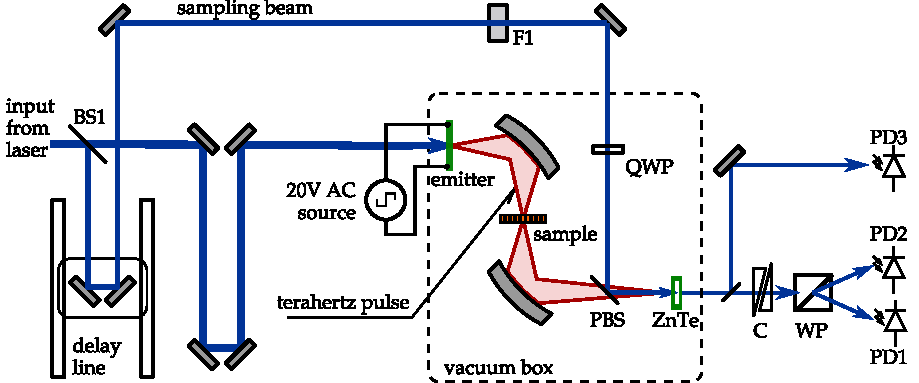
\includegraphics[width=\textwidth]{img/exp_THz_sampling.pdf}
\end{figure}

Before the laser pulse entered the vacuum chamber to induce the photoexcitation of the THz emitter, a small part of its energy was separated by a reflection from a beam splitter (BS1 in Fig. \ref{fg_exp}) into the \textit{sampling} branch. 

The pulse in the \textit{sampling} branch reflected from a pair of mirrors on a delay line, acquiring a precisely controlled relative delay against the terahertz pulse. Then it was attenuated at a filter (F1) and its polarisation was converted from linear to the circular one on a quarter-wave plate (QWP). The pellicle beamsplitter (PBS) directed the optical beam along the axis of the terahertz beam. 

We used the electrooptic sampling mentioned in the previous chapter: The electric field of the terahertz pulse induced a slight transient change in the permittivity tensor of the zinc telluride crystal (ZnTe). The much weaker and shorter optical pulse was modified by this change, acquiring diagonal ellipticity that could be fine tuned for zero signal with the Babinet compensator (C). The Wollaston prism (WP) was used to separate the two diagonal components of the resulting elliptic-polarized light. The difference between these two signals, if a small modulation is assumed, is proportional to the amplitude of the electric field. This allowed us to sample the electric field with a theoretical temporal resolution given by the duration of the optical pulse, but using a standard intensity detection using a pair of silicon diodes.   
%% TODO add references to other papers and theses from our group - one can not describe everything from Gouy shift to PKGraph ...

%}}}
\paragraph{Signal processing and acquisition}%{{{
To reduce the noise, synchronous detection with the \textit{Stanford SRS360} lock-in amplifier was used and the polarity of THz waveforms was modulated by the voltage at the TeraSED emitter. The difference signal at the two photodiodes, PD1 and PD2, was first fed to an analogue filter (with center frequency 91.3 kHz and 3 dB drop at $\pm$ 7 kHz), sampled by the lock-in amplifier and digitally normalized against the signal measured by the auxiliary photodiode PD3. The normalisation was necessary due to the fact that the difference signal is proportional not only to the terahertz field, but also to the laser intensity which may fluctuate over time. 

%The time constant of the lock-in acquisition was comparable to the time which was needed by the delay lines to introduce a picosecond delay. As a result, the speed of delay lines movement suppressed the high-frequency components of the detected signal. Attention must be paid at precise control of the delay line speed and software compensation of the artifacts.

The spectral response of both the emitter and electrooptic sampling substantially influenced the measured sample spectra. Moreover, the phase of the recorded waves was modulated too, as a beam passing through a focus acquires additional phase due to the Gouy shift \cite{kuvzel2010gouy}. Every transmission measurement was therefore normalized in frequency domain against a corresponding free-space reference, so that both the amplitude and phase artifacts cancelled out. 

%}}}

\subsection{Simultaneous reflectance and transmittance measurement}
\paragraph{Principle} %{{{
\label{srtm}
With rearrangement of optics, it would be possible to measure the \textit{reflectance spectrum}, similarly as the transmission was measured. However, due to the complexity of such a setup and its very high sensitivity to the sample displacement, we did not use a second sampling branch for detecting the reflected signal. Instead of using two sampling schemes, we recovered the amplitude and phase reflectance of the sample by stacking it between a pair of thick (3 and 6 mm) sapphire slabs \cite{nemec2012resonant}. Thanks to the relatively high refractive index of sapphire in the terahertz range along the optical axis, $N \approx$ 3.068, these slabs introduce several time-delayed pulse reflections, also called echoes, into the transmitted signal.
%\begin{figure} \caption{A broadband pulse passes through a single layer of microspheres randomly arranged between two sapphire slabs and is sampled by electrooptical detection.}  \centering 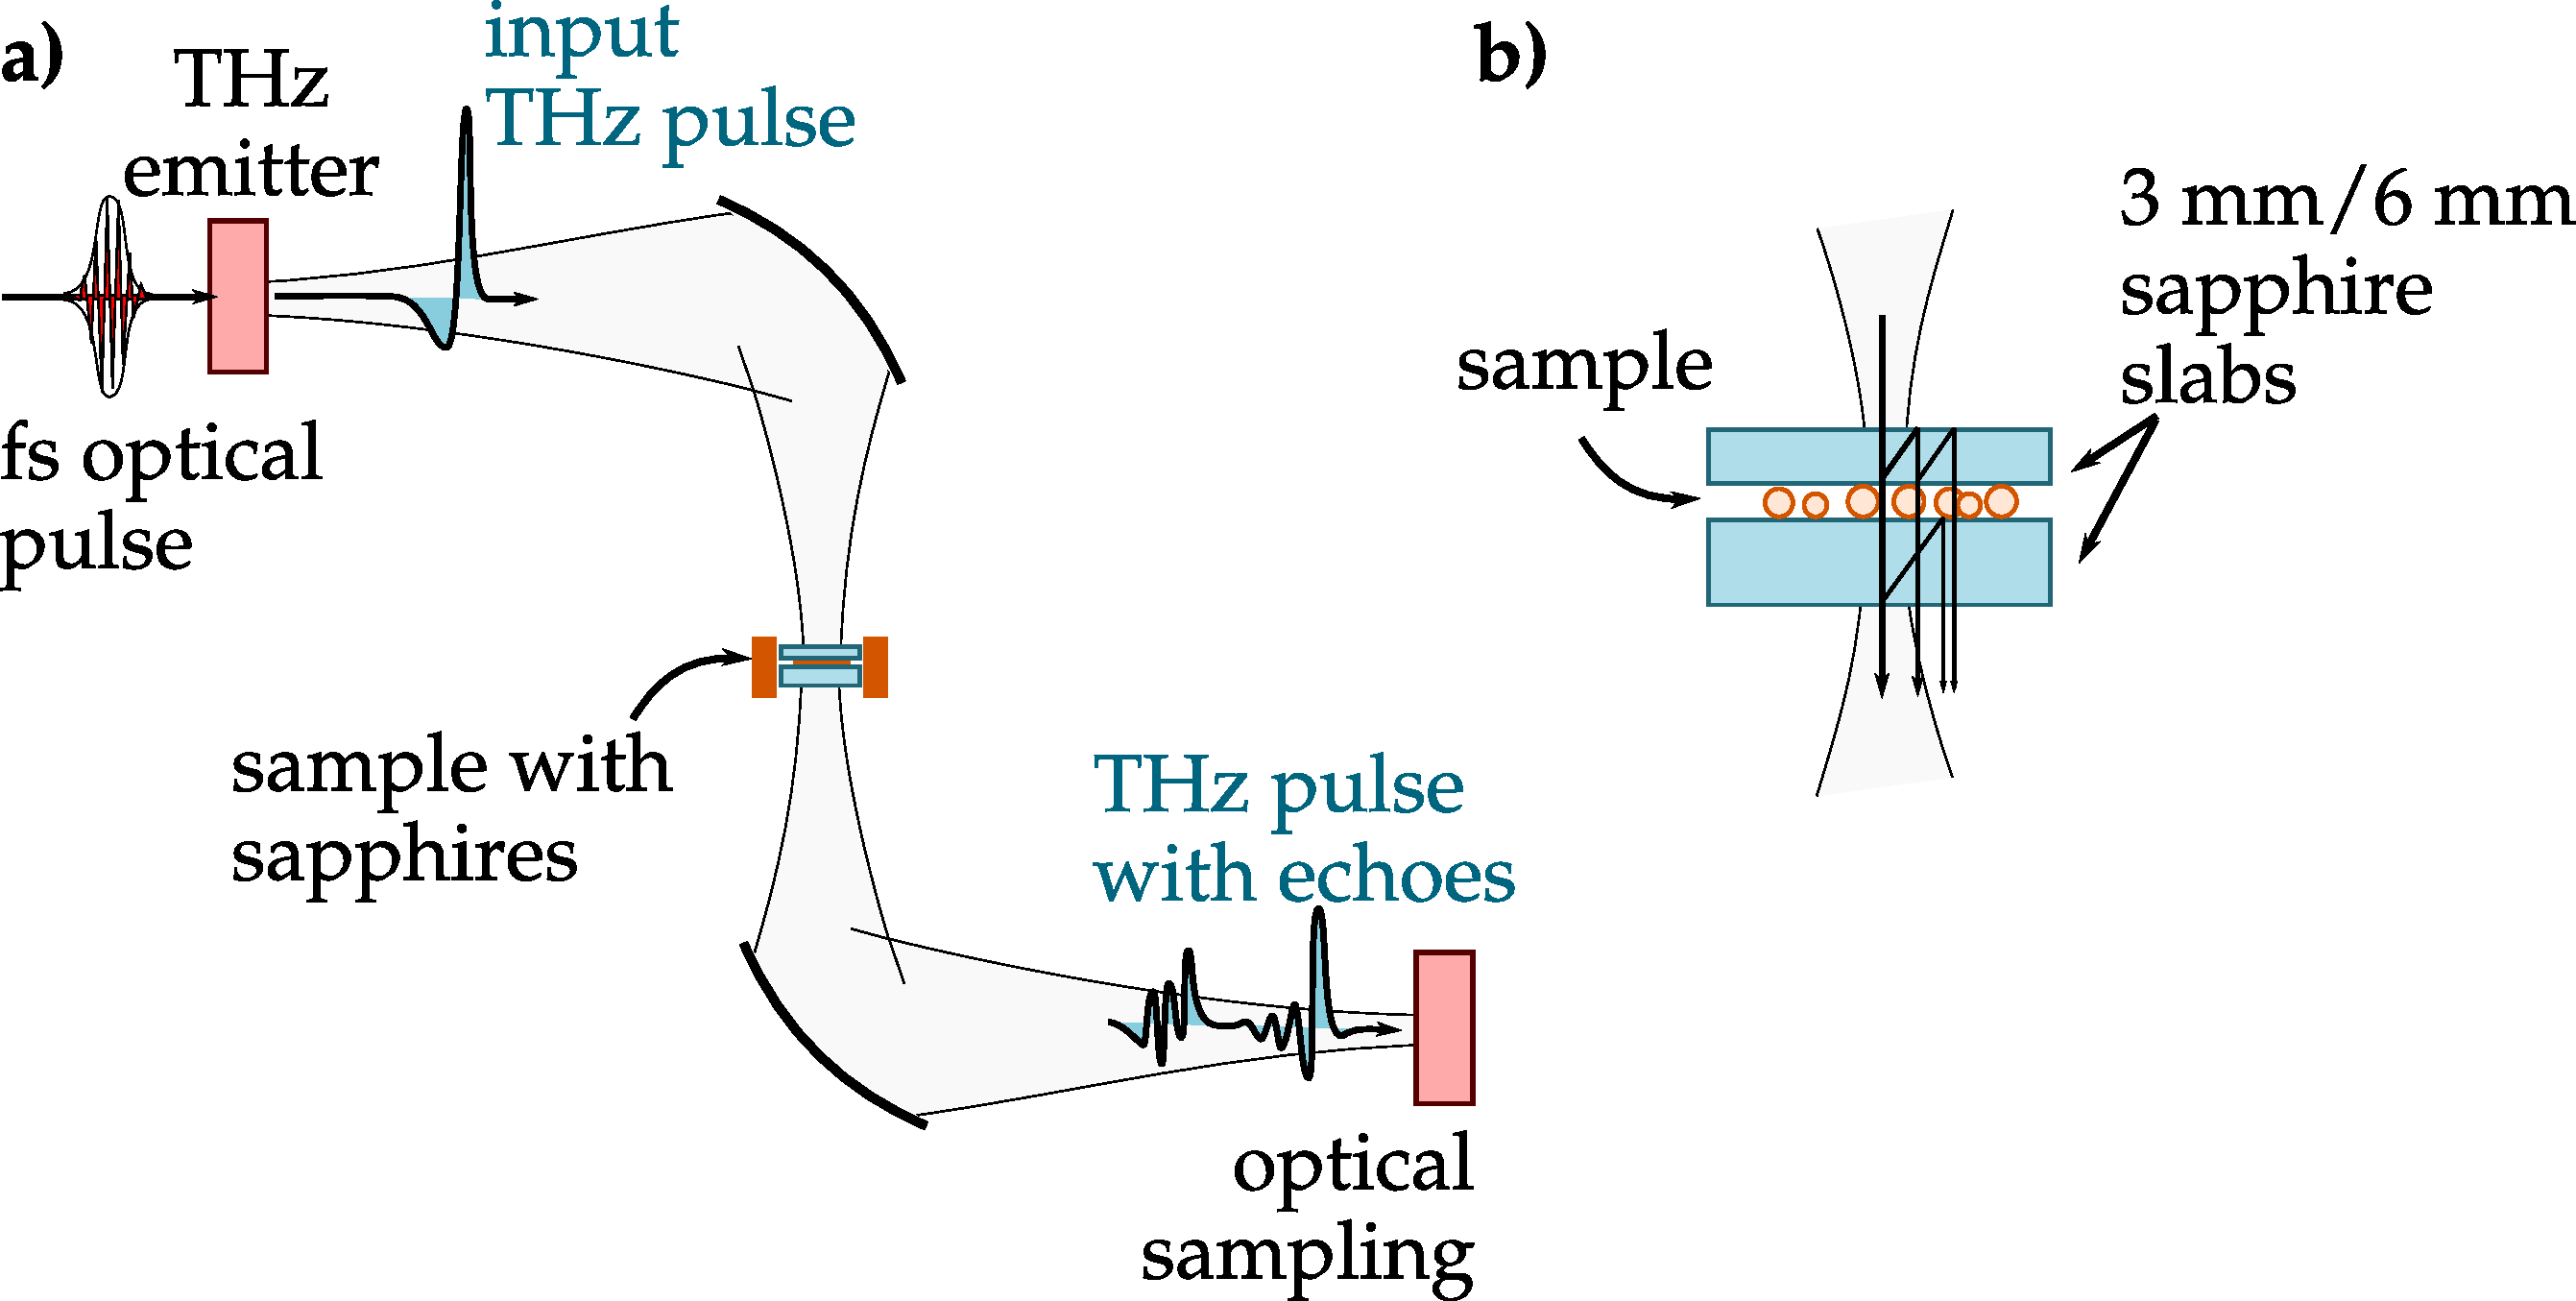
\includegraphics[width=12cm]{img/expe/sample_sapphires.pdf} \end{figure}			%% TODO no use for this figure?

If the beam divergence is neglected, each optical element can be characterised by its complex transfer function in the resulting spectrum. One needs to define three intrinsic transmittance functions: that for the beam passing through the volume of the thin sapphire $A(f)$, the one of the thick sapphire $B(f)$ and one through the thin sample $t_S(f)$; all of these are without the effect of reflection at interfaces. 

The reflection is described by two reflectance functions for the beam reflected on sapphire-air interface $r_{A}(f)$ and on the sapphire-sample interface $r_S(f)$.

By measuring the references of the thin and thick sapphires separately, the spectra of $A(f)$ and $B(f)$ as well as $r_{A}(f)$ can be established \cite{nemec2012resonant}. 

%defines the temporal separation between the main pulse and the first echo.  The reflectance and transmittance of the sample can be simply reconstructed using numerical deconvolution. The results of this method were, unfortunately, less than ideal. Among the reasons may be the possible asymmetry of the studied layer between the slabs, beam divergence and very low signal of both transmittance and particularly reflectance in the stop-bands of the sample.

To retrieve the characteristics of the sample, i.e. $t(f)$ and $r_S(f)$, the overall transmitted time-domain waveform of the sapphire-sample-sapphire structure has to be split into two parts that correspond to the direct pass, and the first echo arising from the pulse reflecting back and forth  in the thin sapphire.
The double propagation delay through 3 mm of the thinner sapphire is roughly 70 ps, which limits the spectral resolution to 14 GHz. All spectral features in the sample transmittance must be significantly broader than this value. Otherwise they could not be resolved, and even more importantly, their temporal ringdown would overlap in the time domain with the following echo and produce spurious results. Using a thicker sapphire could improve spectral resolution of this method, however it conflicts with the requirements of the terahertz beam fitting into the area of the sample \cite{nemec2009tunable} and of reducing the error caused by beam diffraction as noted in the following paragraph.

%}}}
\paragraph{Limitations of the scheme} %{{{
In the experiment, we observed substantial deviation  % TODO add some experimental data to {results} and  reference them here
from the numerically predicted results, which were moreover sensitive to subtle changes in the parameters. We propose  several independent explanations for the experimental errors:
\begin{enumerate}
\item{The geometrical beam divergence can not be fully compensated by the transfer functions of separate sapphire slabs, $A(f)$ and $B(f)$. 
The terahertz beam is relatively tightly focused, and the focus of the echoes is longitudinally displaced compared to the focus of the first pulse. 
The deconvolution algorithm can compensate for slight focus displacement by changing the amplitude  of different frequency components, or shifting them in phase. 

However, due to the hyperbolic shape of the gaussian beam, with its Rayleigh length $z_{R}$ being similar to the sapphire thickness\footnote{As an approximate example, for the main frequency component $f = 1.5$ THz with wavelength $\lambda = c / f \approx 200$~$\upmu$m, for $\vartheta \lesssim 0.15$ rad as an estimated divergence of the beam from its axis, the Rayleigh half-length of a gaussian beam would be $z_{R} = \frac{\lambda}{\pi \vartheta^{2}} \gtrsim 2.8$ mm, i.e. roughly the thickness of the thinner sapphire.}, the overall effect of two sapphires can not be linearly compensated from two separate measurements of each of them.} 
 \item{The possible asymmetry of the sample with regard to the beam axis can substantially bias the measured reflectivity. This happened during the characterisation of the dielectric spheres, when the sapphire distance was defined by a $\approx$60$\upmu$m teflon spacer. The nonuniform size of the resonators required us to attach them to one of the sapphire windows. While the spheres with the 60$\upmu$m diameter were placed symmetrically in the gap, the smaller spheres had an asymmetric position. Since the latter have higher resonance frequencies, the effect of asymmetry was probably also frequency dependent. } 
 \item{The sapphire slabs can influence the near field of resonances in some samples, c.f. Sect. \ref{par_nearfield}. This error should not be significant in transversally homogeneous samples (i.e. slabs), nor in samples that are made of dielectrics with much higher permittivity than that of sapphire. However for some samples, such as metallic resonators, the spectra are be completely changed in the vicinity of a dielectric (see its application on a fishnet sample in Fig. 4.19 in Ref. \cite{yahiaoui2011phd}). }
 \item{Finally, it follows from Eq. (\ref{eq_Neff}) that reliable reflection data can only be retrieved at frequencies where also the transmission amplitude is strong enough for the signal not to be dominated by noise. }
 \end{enumerate}
\label{srtm2}

%}}}

\section{Preparation of the titanium dioxide microspheres}
\paragraph{Fabrication through the spray-dry technique}%{{{
The collaborating laboratory of Dr. Patrick Mounaix in France %% Todo reference to Patrick's group somehow, and mention Oleg Mitrofanow (here, or later)
provided us with high-permittivity TiO$_{2}$ spheres with the sizes from 30 to 100 $\upmu$m, which were examined by the terahertz spectroscopy as dielectric resonators, and as possible constituents of a metamaterial with a negative effective permeability.
\begin{figure}[ht] \caption{Microphotograph of the TiO$_{2}$ spheres after preliminary sieving} \label{fg_microphoto} \centering 
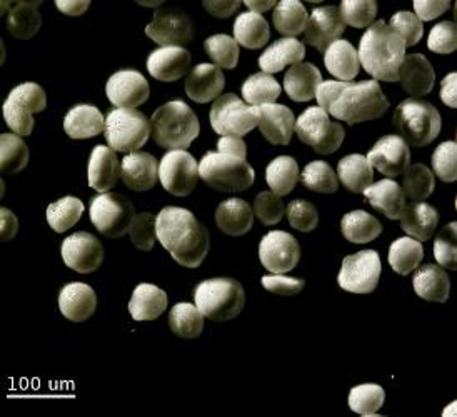
\includegraphics[height=5cm]{img/microscope_TiO2_particles.pdf}
\end{figure}

Compared to most metamaterial designs, the fabrication of the dielectric spheres can be extremely simplified by the \textit{spray-drying}\index{spray-drying technique} technique. In contrast with the expensive and time consuming \textit{top-down} processes such as laser cutting, litography or polishing, this is a typical \textit{bottom-up} process, where the particles are formed all within one procedure, though certain postprocessing is needed. 

As a first step, rutile (TiO$_{2}$) was ground to a sub-microscopic powder \cite[pp. 91-93]{yahiaoui2011phd}. A suspension of this powder in ethanol was sprayed into flame. It immediately formed spherical droplets, which dried up and sintered in the hot air. Rutile concentration in the suspension, feed rate and gas flow in the flame determined the average size of the sintered particles.

The resulting particles were annealed in a furnace to further solidify. The degree of recrystallization could be controlled  by the temperature of the furnace from 1200 to 1400 $^{\circ}$C from microscopic grains to few large crystalline domains in one microsphere. Note these temperatures used are still far below the melting temperature of rutile, which exceeds 1800 $^{\circ}$C.
Similar TiO$_{2}$ microspheres are also available commercially (e.g. from Brace, GmbH), and were likely made with a similar process.

The annealed spheres were further treated with the aim to break or eliminate clusters, by means of light milling with agathe mortar, which was separated afterwards by ultrasound bath cleaning in ethanol. Pre-sieving was performed on commercial sieves with 100, 53, 50, 40 and 38 $\upmu$m size of the square hole, though these nominal parameters of sieves should be in no way understood as hard limits for the particle sizes. The procedure of milling, cleaning and sieving was repeated 2-3 times, according personal communication with Dr. Patrick Mounaix and {Dr.} U-Chan Chung.

Only the low-temperature annealed samples were measured by the terahertz spectroscopy in this thesis. The fine-grained rutile was assumed to represent a nearly isotropic dielectric. We estimated the size of the constituent crystalline grains by grinding one microsphere and observing it under a polarizing microscope: unlike polycrystalline aggregates, small rutile monocrystals appear as coloured particles due to their inherent birefringence. In this way, the sizes of crystalline grains were assessed to be in the order of few micrometers or smaller.

%\textit{
%(\ldots) As the spheres have been sintered at high temperature, they have been separated from a platinum plate with a small soft paintbrush followed by a light milling with a agathe mortar. The goal was to separate the spheres that are welded to their neighbours due to the sintering step. All the spheres were treated in ultrasound bath using ethanol as a liquid phase. After natural drying, the sieving was performed. (\ldots) square (or rectangular) holes sieves were used. The meshes used were 106, 100, 53, 50, 40 and 38 micrometer. As a dry sieving step was performed, the particles were light milled again in order to try to break possible agglomerates which would not go through the mesh. This process was repeated 2-3 times and a final wet sieving with ethanol was performed in order to "wash" the spheres. No special measures were taken according to their shapes. (\ldots) } 
% TODO


%}}}
\paragraph{Theory of anisotropic sieves}%{{{
Triple sieving on commercial sieves, weaved from stainless steel wire, did not provide narrow enough size distribution, which is however essential for obtaining a narrow resonance peak of the sample. We therefore developed a more exact method for very fine sample sieving and characterisation. 

\begin{figure}[ht] \caption{Correspondence between the hole shape (above) and the set of ellipsoids that can pass through the hole (below), determined by their medium and minor axes. Somewhat surprisingly, the \textbf{(a)} square and \textbf{(b)} lozenge holes result in circular/elliptic set of passing particles, whereas the \textbf{(c)} circular and \textbf{(d)} elliptic holes result in the square/rectangular shape of such an region.\\
For clarity, some limiting-case examples of the ellipsoid projection and the equivalent position on the minor-major ellipse axis plot are drawn in blue, violet and red. } \label{fg_sieve_pass_notpass} \centering 
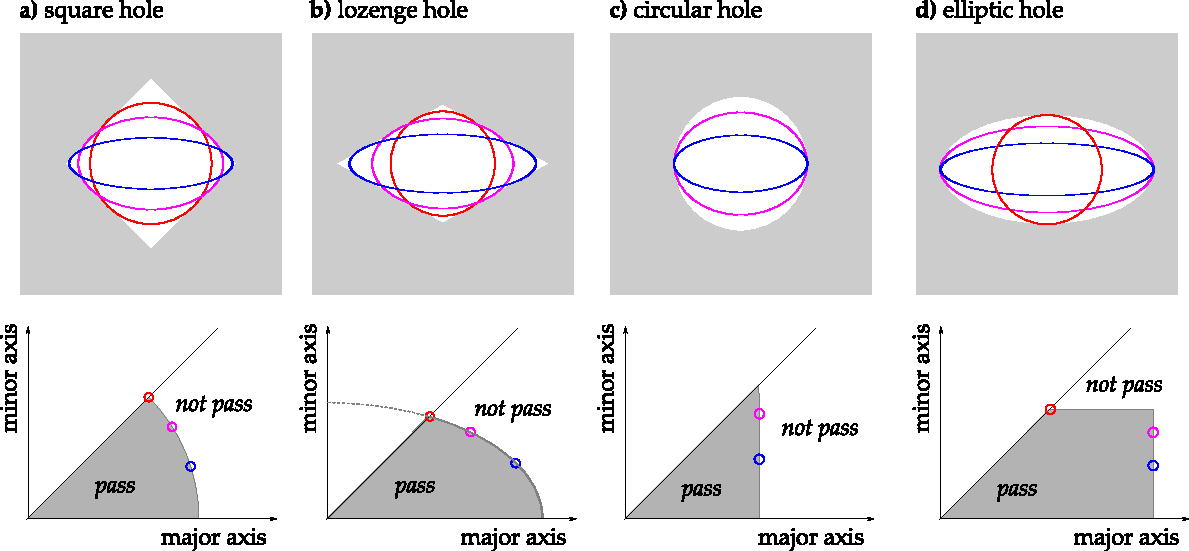
\includegraphics[width=\textwidth]{img/technology/sieve_pass_notpass.pdf}
\end{figure}
In the following, the dielectric particles are approximated by ellipsoids with three (generally different) half-axes $$\rho_a \leq \rho_b \leq \rho_c.$$ For the purpose of sieving, only the values of the shortest two half-axes, $\rho_a$ and $\rho_b$, decide whether the particle can pass through the sieve. The longest ellipsoid half-axis $\rho_c$ does not affect this, although it may influence the sieving speed. Therefore we can represent each three-dimensional particle with its projection on the smallest possible ellipse, which is described by its \textit{minor axis} $\equiv 2\rho_a$, and by its \textit{major axis} $\equiv 2\rho_b$ (which is, in fact, the \textit{medium axis} of the ellipsoid). For a given shape of a hole in a homogeneous flat sieve, it is easy to determine which values of minor and major ellipse axes allow a particle to pass through, and which not. For a square sieve such area in the parameter space forms a disk around the center of origin (Fig. \ref{fg_sieve_pass_notpass}a). It can be shown that when the sieve is diagonally stretched, forming a lozenge-shaped hole, the area of spheres allowed to pass transforms into an ellipse (Fig. \ref{fg_sieve_pass_notpass}b). When the hole shape is circular or elliptical, it is obvious that the area forms a part of a square or of a rectangle, respectively  (Fig. \ref{fg_sieve_pass_notpass}c,d).

The resonance frequency of a dielectric resonator depends on all three half-axes, $\rho_a \leq \rho_b \leq \rho_c$. In order to select a size fraction as narrow as possible, one has to use double sieving: the above sieve not allowing the fraction of particles too big, the bottom sieve removing the fraction of particles too small. This is where the anisotropic hole shapes become useful -- the bottom sieve can exclude also all oblong particles with the difference of $\rho_a \leq \rho_b$ too big. This effect is illustrated in Fig. \ref{fg_double_sieving}, which also presents a comparison between using more usual sieves with square/lozenge holes and the approach with a pair of sieves with micromachined square/elliptical holes. Obviously, the latter approach better discriminates between the \textit{shapes} of the ellipsoids. This advantage further gains on importance when the anisotropy of the sieve is low.

\begin{figure}[ht] \caption{Application of the effect from Fig. \ref{fg_sieve_pass_notpass} for separating a narrow fraction of ellipsoids between the sieves. Both combinations of \textbf{(a)} square-rectangular and \textbf{(b)} circular-elliptic sieves can be used, with the latter one promising better selectivity also in terms of the particle aspect ratio.} \label{fg_double_sieving} \centering 
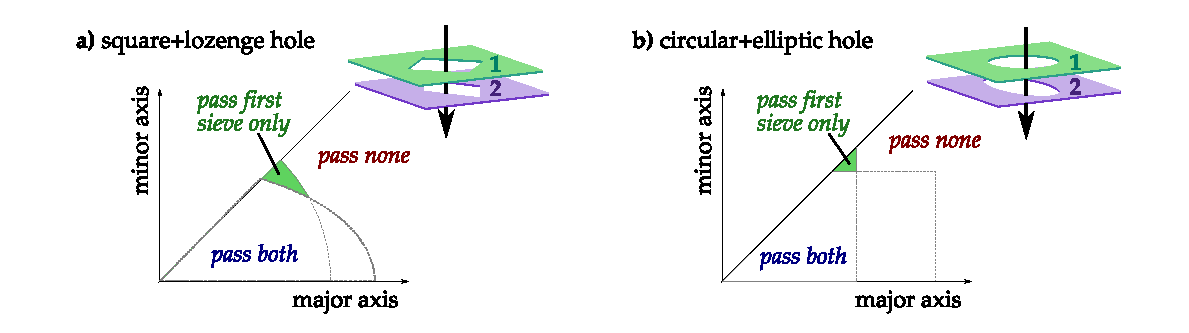
\includegraphics[width=\textwidth]{img/technology/sieve_double_sieving_fractions.pdf}
\end{figure}
It shall be noted that although we plotted a binary (pass/not pass) function in Figs. \ref{fg_sieve_pass_notpass} and \ref{fg_double_sieving}, the sieving speed continuously drops when the particle dimensions approach those of the sieve holes. 
%For any finite sieving time, this obviously affects the statistics of particles passing the sieve, favoring the average size to be lower for short sieving times.
However, this particular fraction of particles is exactly what one is interested in during the high-accuracy sieving. The process must therefore be run for a long enough time, of the order of days, and with as high a sieving speed as possible.
%}}}
\paragraph{First sieving apparatus}%{{{
%Finally, they were carefully sieved in many iterations, to select a size fraction as narrow as possible.
Employing the idea of anisotropic sieves from Fig. \ref{fg_double_sieving}a, the author assembled a first prototype based on nylon sieves, as depicted in Fig. \ref{fg_sieving1}. Two glass containers, 6 mm high and 11 mm in diameter, were cut on a lathe from a glass tube. On their bottom, the sieves were glued and carefully clipped. The side of the sieve holes was 60$\pm$5 $\upmu$m. 

The mesh was woven of nylon threads, so the bottom sieve could easily be stretched by ca. 20-25 \% in the diagonal direction.  The above sieve was kept isotropic. 

This  property however prove to be also detrimental for precise sieving, as the threads easily bent aside under only a small force, thus allowing oversized particles either to pass or to get stuck permanently and to block the sieve within few minutes. To help resolving the latter problem, two additional narrow glass rings were cut from the glass tube, supporting much coarser sieves with 150 $\upmu$m pitch glued on the bottom, to allow little spherical springs bounce beneath the sieves and to loosen the particles that got stuck in the holes. For the same purpose, 2mm plastic balls were added to the microsphere samples.  

A cover on top prevented the particles to jump out of the above container. The whole stack was carefully lowered into a test tube with a greater diameter, and vibrated by a tiny electric motor glued on the bottom.

\begin{figure} \caption{\textbf{(a)} Photograph and \textbf{(b)} scheme of the first sieving apparatus based on square-lozenge sieve pair, with a schematic out-of-scale illustration of its operation for an input of four different microspheres \textbf{(c)}}  \centering 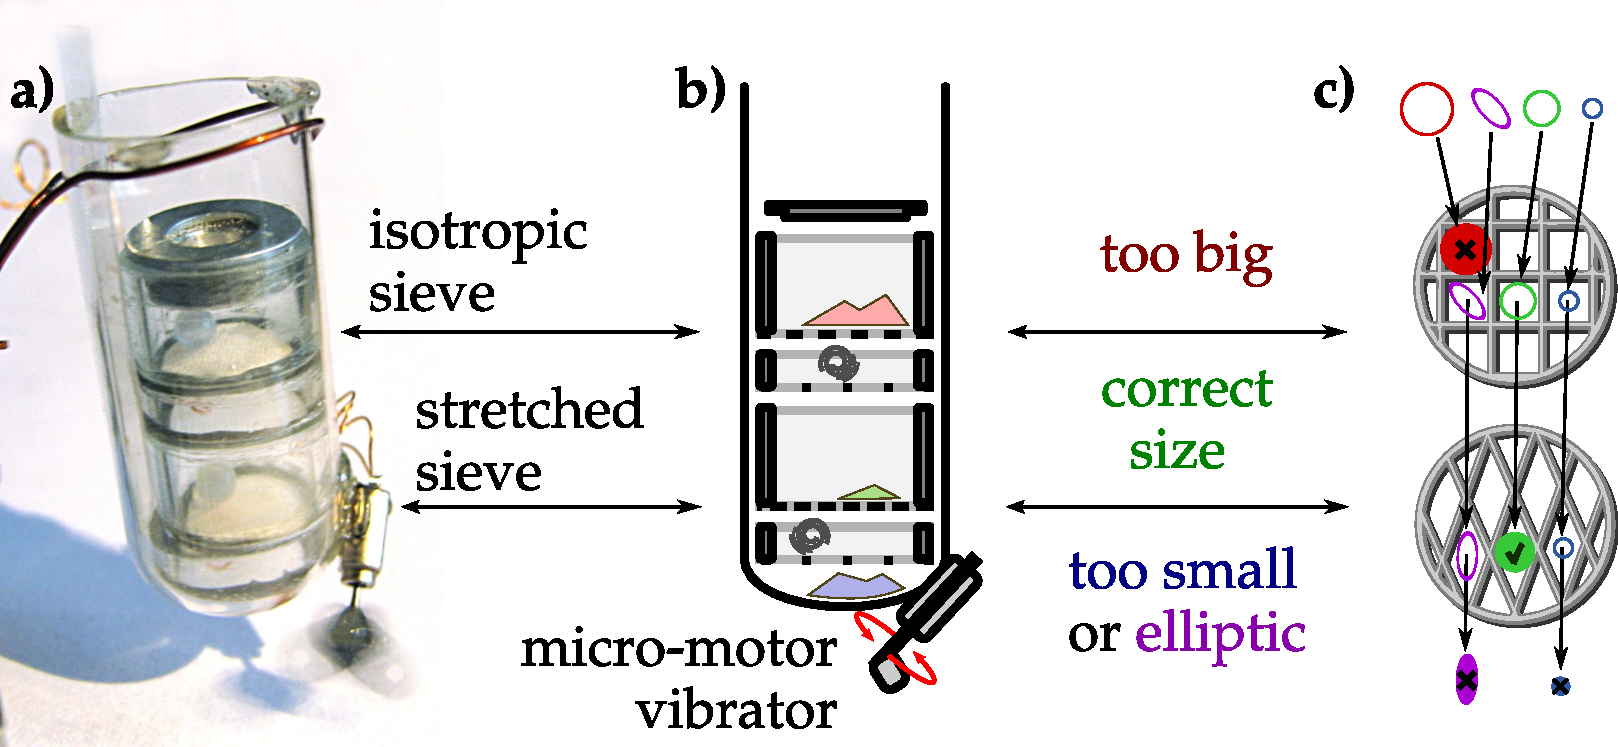
\includegraphics[width=12cm]{img/expe/sieving1.pdf} \label{fg_sieving1} \end{figure} 

%}}}
\paragraph{Second sieving apparatus}%{{{
\begin{figure}[ht] \caption{\textbf{(a)} A sketch of the acoustic sieving device, and \textbf{(b)} a photograph thereof} \label{fg_sieving2} \centering 
	\begin{overpic}[height=.4\textwidth]{img/technology/sieve2_sieving_scheme.pdf}  \put(-10,93) {\textbf{(a)}} \end{overpic}
	\begin{overpic}[height=.4\textwidth]{img/technology/sieving_m.pdf}              \put(1,85) {\textbf{(b)}} \end{overpic}
\end{figure}
The partially promising results and, more importantly, obvious deficiencies of the previous apparatus motivated the construction of a second one depicted in Fig. \ref{fg_sieving2}.
Different from any other sieving apparatus known to the author, this one made use of vertical acoustic waves for the movement of particles. It consisted of two coaxial glass tubes: The inner tube, with outer diameter of 13 mm, had a round metallic sieve glued to its bottom, and on its upper end it was covered by a small acoustic transducer. The outer tube (90 mm long, outer diameter 26 mm) surrounded the inner one and had a round bottom, where the particles were collected. 

The gaskets ensured that the whole apparatus was tightly closed, preventing both sieved particles and the sound from escaping. The brass ring with the transducer was fixed to a massive aluminum stand, and the rest of the structure was held by two accessible screws that allowed easy disassembling. 

The key advantages of this novel approach are the following:
\begin{enumerate}
 \item{The speed of sieving is expected to grow with the frequency at which the particles hit the sieve. The acoustic frequency of 1 kHz is roughly two orders of magnitude higher than in usual commercially available devices. Moreover, the spheres are  continuously stirred, so it is ensured that a layer of over-sized particles does not occupy the sieve.} 
 \item{The upward air pressure pulls out particles that got stuck in the sieve in every period of acoustic vibration. This resolves the major issue of clogging inherent for the previous prototype.} 
 \item{Avoiding macroscopic vibrating parts, except the membrane of a small acoustic transducer, allows the device to operate over multiple days with reduced risk of mechanical failure.}
 \end{enumerate}
The outer tube acted as an acoustic resonator, greatly enhancing the effect of the sound when tuned to resonance around 750-900 Hz. These frequencies obviously correspond to the fundamental acoustic resonance, as the corresponding quarter-wavelength is close to the 10 cm length of the outer tube.  The electrical input power of the sine wave feeding the device was in the order of 1 W.

%}}}
\paragraph{Sieving challenges}%{{{
A practical deficiency of this setup was that the upper opening of the transducer radiated relatively intense sound during operation. We resolved this potential issue by covering the whole apparatus by a robust glass bell jar.

With the acoustic power and frequency correctly adjusted, the particles formed a cloud 5--10 mm high. One difficulty arose from that the small particles tend to attach to the surface of glass or metal, probably due to electrostatic charges on their surface. While at an average particle radius $\rho = 50$ $\upmu$m this effect was rather marginal and transient, it took only few seconds of sieving for $\rho = 20$ $\upmu$m particles to immobilize permanently on any surface. It has however proven efficient to tap the upper brass ring, as the mechanical shock released most spheres and renewed the sieving process. To ensure unattended sieving for a timespan in order of days, we added a little motorized hammer with a timing circuit (Fig. \ref{fg_sieving2}a).

The amount of particles in one batch was limited to ca. 10--20 mm$^{3}$, otherwise the sieve would be covered with a layer too thick, which could not be efficiently lifted by the acoustic pressure.
This problem could however be slightly mitigated by tilting the apparatus. With a tilt of 5--10 degrees, the bulk of particles then accumulated near one side, leaving most of the sieve surface free for sieving the moving particles. Given the small amount of particles required for the terahertz spectroscopy measurements, it is however advisable to sort a batch in order of 1--3 mm$^{3}$.

%}}}
\section{Optical determination of microparticle statistics}
\paragraph{Image preparation} %{{{
An accurate characterisation of the particle statistics was necessary not only to assess the efficacy of sieving, but also to explain  on a quantitative basis possible differences between the measured terahertz spectra and the computed ones. To obtain reliable statistics, thousands of particles needed to be evaluated, repeatedly for every sample. This, along with the small dimensions of particles, indicated that the most viable way to do so would be the optical microphotography with computer image processing automatically resolving each particle.

Computer \textit{granulometry}\index{granulometry}, identification and measurement of photographed particles from a digital image,
is a well-established technique. It is implemented in several advanced image processing programs, of which \textit{ImageJ} was selected \cite{abramoff2004image} since it is free of charge and allows its use for large batches of images through the use of macros. 

The transmission microphotographs were acquired either with the lowest magnification on a laboratory microscope, or with a portable microscopic digital camera on its highest magnification, yielding similar results.

The first processing step, applied at the somewhat blurred photographs, as shown in Fig. \ref{fg_sievingstats}a, was to establish the intermediate brightness level between the image's bright and dark areas, and apply a threshold so that the image was a binary function. Then the \textit{ImageJ}'s \textit{watershed} algorithm was applied to relatively reliably resolve two or more touching particles, and a particle outline was found. An example is depicted as cyan lines in Fig. \ref{fg_sievingstats}b. Finally, the particle outlines were approximated by best matching ellipses, and the major and minor axes of the ellipse were added into the statistics. 
\begin{figure}[ht] \caption{\textbf{(a)} A small section of a microphotograph of a pre-sieved sample before applying the described double-sieve method, \textbf{(b)} the corresponding identification of particles in ImageJ} \label{fg_sievingstats} \centering 
	\begin{overpic}[height=.30\textwidth]{img/technology/imagej_photo.pdf} \put(-9,72) {\textbf{(a)}} \end{overpic}\quad\quad
	\begin{overpic}[height=.30\textwidth]{img/technology/imagej_found.pdf} \put(-9,72) {\textbf{(b)}} \end{overpic}\quad\quad
\end{figure}
We complemented the \textit{ImageJ} macro with a Python script enabling us to process multiple photographs in a batch, and to plot the resulting histograms of the ellipse axes distribution. The script has also been published online \cite{dominec2014_imagej}. The scale for each batch of images had to be determined from a separate photograph of a ruler.

%}}}
\paragraph{Imprecision of the method} %{{{
An intrinsic deficiency of this method is that it was not possible to resolve the third dimension of particles. 
It can be however estimated that when % TiO$_{2}$ 
ellipsoidal particles were randomly sprinkled on the glass, they would lie mostly on their flat side -- i.e. their orientation would enable to measure the \textit{medium} $\rho_b$ and \textit{major} axes $\rho_c$ of the ellipsoid. This is in contrast with the process of sieving, as described above, where the particles were sorted according to their and \textit{minor} $\rho_a$ and \textit{medium} $\rho_b$ axes. 

This source of error is probably similarly important as another one, arising from rough shapes of the particles which could not always be well approximated by an ellipsoid. 
%\todo{add the previous and resulting statistics? the THz spectra should better go to the Results }
%}}}

\section{Laser cutting}
\paragraph{Fabrication of dielectric bars}%{{{
Dielectric or metallic structures can be made by cutting a thin polished slab of the given material. Electromagnetic waves with a frequency of  1 THz have a free-space wavelength of 0.3 mm. Periodic structures designed to operate in this range have their unit cells of a similar size or less, and their finest features are usually in the order of 10-20 $\upmu$m. 

The sample already shown in Fig. \ref{fg_STO_bar_rt} consisted of bars from strontium titanate (SrTiO$_{3}$) with a rectangular cross-section (see Fig. \ref{fg_STO_bar_geom}), where a structure with 10--30 $\upmu$m lateral bar dimensions was engraved into a thin slab of the dielectric of a similar thickness \cite{yahiaoui2011tunable}.

If the slab consists of a monocrystal or a ceramic, it is usually extremely brittle and also sensitive to breaking due to thermal stresses. Femtosecond laser cutting (or, micro-machining) is suitable for such a task because it delivers the energy so fast that most of the heated material evaporates before the heat can diffuse into the rest of the structure. 
The strontium titanate bars were fabricated by the \textit{Alphanov} facility in France.

%}}}
\paragraph{Fabrication of sieves and fishnets}%{{{
Femtosecond cutting of metallic sheets into two-dimensional meshes is relatively easy,   
compared to the dielectrics, 
and was implemented in our laboratory. To achieve the required precision, we used 20 or 30 $\upmu$m thick high-quality stainless steel foils. 

The femtosecond laser used was different from that serving as the femtosecond source for terahertz spectroscopy (Sect. \ref{sect_tdts}). A largely sufficient power was provided by the \textit{Spectra Physics Spitfire Ace} multipass titanium-sapphire amplifier, with 1 mJ of energy per impulse, duration of $\sim$50 fs, and 5 kHz repetition rate. Its output beam had to be attenuated to obtain finer cut at the expense of a slightly slower speed. The mechanical part consisted of two crossed \textit{Owis} stepper-motor controlled linear stages, and a fast mechanical shutter allowed us to control the beam with a sufficient resolution of ca. 100 ms. 
\begin{figure}[ht] \caption{\textbf{(a)} Laser cutting the steel foil with a moving holder for four samples, metal vapour ventilation, and the focusing lens. Bright plasma spot is visible at the focus. \textbf{(b)} The resulting sieves made from 30 $\mu$m stainless steel foil with 10 mm overall diameter.} \label{fg_microfab} \centering 
	\begin{overpic}[height=.35\textwidth]{img/technology/sieve2_drilling_m.pdf} \put(-8,82) {\textbf{(a)}} \end{overpic}\quad\quad
	\begin{overpic}[height=.35\textwidth]{img/technology/steel_sieve_on_paper.pdf} \put(-8,80) {\textbf{(b)}} \end{overpic}
\end{figure}

The 3 mm wide beam was focused by a lens with a focal length of 10 mm or 50 mm (Fig. \ref{fg_microfab}a). The tighter focusing lead to a better resolution, but had stricter requirements for accurate focusing of the beam. To facilitate the task of optimal focusing, we devised a focusing-collimating setup which used the fact that  the  steel foil reflected the light like from a point source only when it was exactly in the lens focus. Then the reflected light would be collimated again by the very same lens into a beam returning to the laser. 
%the reflection would not be collimated if the reflection occurred in front of the focal plane or behind it. 
A part of the reflected beam energy was reflected sideways by a skewed glass in front of the lens, so that one could finely align the lens seeking for the smallest spot diameter on a distant screen.

A compact stepper-motor controller of a custom design \cite{dominec2015_triostepper} facilitated to automate the sample movement by means of computer control operated by a Python script. The sequences of shutter opening, sample movement and shutter closing could be assembled into a program for fabrication of a whole mesh sample of ca. 10 mm diameter, which took about 30 minutes to finish. Multiple different meshes with different parameters could be cut out from one steel foil in a batch, without user interaction.

%}}}
\paragraph{Laser cutting issues}%{{{
The metal evaporated during the laser cutting immediately oxidises in the air. Although in total only few milligrams of the stainless steel foil were removed, the microscopic particles would pose a risk of damaging optical components. We built a miniature ventilation and filtering system out of a tube filled with cotton wool and fine synthetic fibers. After few meshes were cut, the cotton changed its colour from white to pale brown, indicating that at least a part of the particles were filtered out.

A greater challenge arose from thermal expansion of the foil. In order to fully utilise the valuable laser beam time, one would wish to set the cutting speed as high as possible. However, the speed of cutting was rather limited by the speed of stepper motors. The heat remaining in the steel foild was high enough to cause its thermal expansion and bending out of the plane of its holder. Even though the resulting displacement was less than 1 mm, the sheet moved significantly out of the beam focus. We assume this was the reason for slight variations between the hole sizes in Fig. \ref{fg_fishnet28_photo}. The effect would be diminished through slower cutting speed or by gluing the foil to a sacrificed rigid substrate.

Cutting the foil into free-standing wire array was however not successful since the resulting thin wires bent out of their original plane due to the thermal expansion. Their spacing was so uneven that no usable sample of wires was made.

%}}}
\paragraph{Difference between sieves and fishnets}%{{{
The meshes were made for two purposes -- either as sieves used in the second sieving apparatus described above, or as metamaterial samples known as \textit{fishnets}\index{metamaterial!fishnet!fabrication}, which are predicted to exhibit a negative index of refraction (see Sect. \ref{section_fishnet}). The difference between these applications is subtle; the meshes intended as sieves would surely exhibit a resonance in the terahertz range. 

The optimum  size range for the titanium dioxide spheres resonating around 1 THz is around 30--60 $\upmu$m, which determined the hole diameter of sieves. To maintain mechanical robustness, the periodicity in sieves was kept much larger than the hole diameter, usually 300$\times$300 $\upmu$m, and the thickness was chosen as 20 or 30 $\upmu$m.
The fishnets had the same periodicity as sieves, and the hole dimensions were chosen between 150 and 280 $\upmu$m. 
For cleaner cutting, a thinner stainless foil was used, with a thickness of 5 $\upmu$m.

% TODO
%To achieve the required precision of sieving, we fabricated the sieves by femtosecond laser drilling of 20--30 $\upmu$m thick stainless steel steel foil
%These sieves then were employed in a device that subjected the microsphere sample to acoustic vibrations, improving the speed of the demanding sieving process to acceptable level

%}}}

